\section{Обзор}
\subsection{Синтаксический анализ графов}
Графы имеют множество применений в различных областях науки и производства. Примером использования графов являются графовые базы данных.

При работе с графами возникает необходимость выполнения запросов поиска по ним. Задача выполнения таких запросов формулируется как поиск всех возможных путей, удовлетворяющих заданным ограничениям. Ограничения задаются, как правило, регулярной грамматикой, однако наиболее лаконично и выразительно такие запросы можно представить с помощью контекстно-свободной грамматики. Контекстно-свободная грамматика (КС-грамматика) $G_1$ представляет собой множество правил грамматики $P$, нетерминальных $N$, терминальных $T$ и стартовых символов $S$. Пример грамматики представлен на листинге~\ref{grmG1}.

\begin{listing}
\caption{Грамматика $G_1$}
\label{grmG1}
\centering
$\begin{array}{ll}
E \rightarrow N \ + \ N \ | \ N \ - \ N
\\
N \rightarrow a
\end{array}$
 \end{listing}

В примере символы $E$, $N$ – нетерминальные символы, «–», «+», «a» – терминальные, $E$ – стартовым символом. Итак, задача выполнения запросов является задачей поиска в ориентированном графе всех путей, представляющих собой строки языка, заданные КС-грамматикой. Одно из возможных решений такой задачи – это модификация алгоритмов обобщенного синтаксического анализа строк, которые строят все деревья вывода для данной строки. В данных модификациях вывод строк строится во время обхода входного графа в ширину, при этом для путей, соответствующих строкам, принадлежащих входному языку, осуществляется построение деревьев разбора в виде компактного представления леса разбора SPPF. Деревья разбора, представленные в таком виде позволяют получить дополнительную информацию из результата, а также производить семантические действия над ними.

Примером модификаций алгоритмов синтаксического анализа для синтаксического анализа ориентированных графов является алгоритм, основанный на алгоритме Эрли~\cite{Sevon}. Данный алгоритм позволяет записывать запросы к графовым структурам данных с указанием направления поиска: прямое направление, когда поиск производится в направлении ребер графа, или обратном – по обратным ребрам. Однако в рассматриваемой реализации необходимо указывать максимальную глубину обхода. Это не удобно, когда мы не знаем точной глубины, которой нам нужно производить анализ. Результат получается ограниченным, возможно потеря некоторых решений. Результатом работы алгоритма является подграф, содержащий пути разбора. 

Другим примером синтаксического анализа графов является алгоритм основанный на RNGLR~\cite{RNGLR}. Он позволяет получить лес разбора для регулярно аппроксимируемого набора входных строк, представляющего собой граф.

 Последним примером является решение основанное на алгоритме нисходящего анализа GLL~\cite{GrigRagCFPQuerying}. Данное решение позволяет производить анализ любого графа и при этом результатом работы является такая структура данных как бинаризованный лес разбора Binarized Shared Packed Parse Forest~\cite{SPPF}. 

 Shared Packed Parse Forest – это граф, компактно представляющий множество деревьев разбора. Компактность достигается переиспользованием общих поддеревьев разбора, за счет чего удается сократить расход памяти до $O(n^3)$, где n — длина входной строки. В отличие от обычного дерева разбора, которое содержит в себе только терминальные и нетерминальные узлы, в SPPF были введены дополнительные типы узлов: упакованный узел (packed node) и промежуточный узел (intermediate node). Упакованный узел создаётся при возникновении неоднозначностей, а промежуточный узел — для хранения промежуточных состояний в бинаризованном SPPF. SPPF — это ориентированный граф, который может иметь циклы. Для того чтобы поиск в таком графе происходил за $O(n^3)$, было введено дополнительное условие для построения SPPF: он должен быть бинаризованным. На рис.~\ref{fig:sppfV} представлено, как выглядит SPPF, состоящее из деревьев на рис.~\ref{fig:sppfA} и рис.~\ref{fig:sppfB}. А на рис.~\ref{fig:sppfG} представлена его бинаризованная форма. Пример взят из статьи~\cite{IzmCombinator}.

 \begin{figure}[t]
 \centering
    \subfloat[Дерево разбора 1]{
        \label{fig:sppfA}
        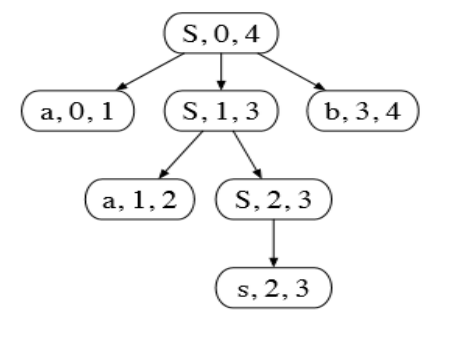
\includegraphics[width=0.35\textwidth]{Smolina/pics/SppfA.png}
    }
    \subfloat[Дерево разбора 2]{
        \label{fig:sppfB}
        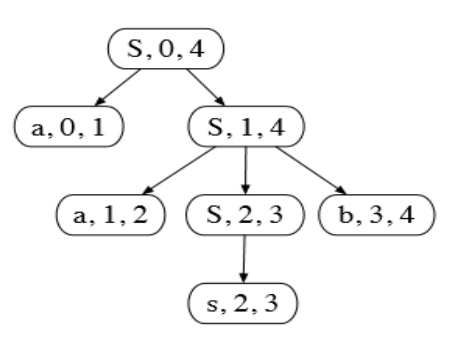
\includegraphics[width=0.35\textwidth]{Smolina/pics/SppfB.png}        
    }

    ~\\~
    \subfloat[SPPF]{
        \label{fig:sppfV}
        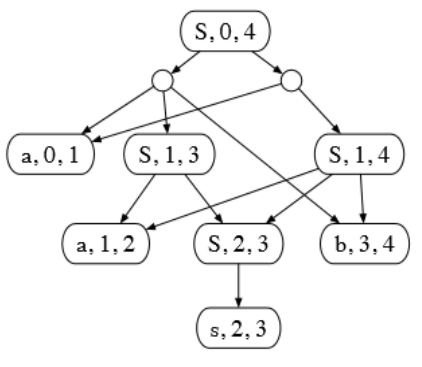
\includegraphics[width=0.35\textwidth]{Smolina/pics/SppfV.png}        
    }
    \subfloat[Бинаризинное SPPF]{
        \label{fig:sppfG}
        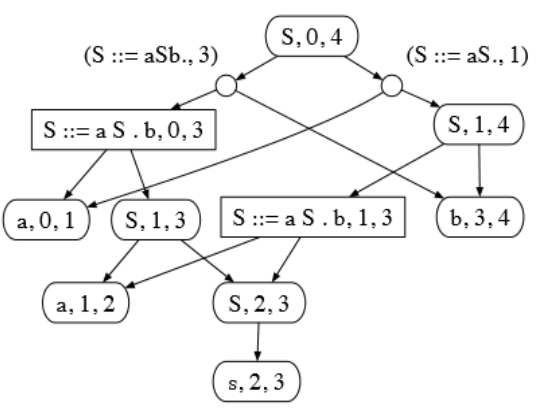
\includegraphics[width=0.45\textwidth]{Smolina/pics/SppfG.png}        
    }
 \caption{Преобразование леса разбора к виду SPPF}
\end{figure}

Решение на RNGLR и GLL построено на основе генерации синтаксических анализаторов. Такое решение не является удобным при работе с графами и графовыми базами данных, так как при добавлении малейших изменений необходимо генерировать руками новый синтаксический анализатор. 

В сфере промышленных графовых баз данных существуют свои решения для запросов. Для каждой из них разрабатывается свой язык для запросов. К примеру для графовой базы данных Neo4j~\cite{Neo4j} существуют языки записи запросов Cypher~\cite{Cypher} и openCypher~\cite{openCypher}, а для OrientDB~\cite{OrientDB} используется язык SQL~\cite{Sql}. Они не поддерживают формат запроса в виде контекстно-свободной грамматики. Более того, нет возможности получить все возможные деревья разбора по записанному запросу.

 Таким образом, нашей целью стала разработка решения, в котором грамматику можно было специфицировать в самом коде целевого приложения. Один из возможных подходов к решению данной задачи — использование техники парсер-комбинаторов~\cite{HOFunParsing}.

\subsection{Техника парсер-комбинаторов}
Комбинатор — это функция высшего порядка, которая из набора функций строит новую функцию. Возможность принимать функции на вход, комбинировать и возвращать их является отличительной чертой функциональных языков программирования, где комбинаторы моделируются функциями высшего порядка.

Парсер-комбинатор — это функция высшего порядка, которая на вход получает множество синтаксических анализаторов и возвращает новый синтаксический анализатор. 

Для синтаксического анализа необходимо научиться анализировать элементарные сущности (терминалы, нетерминалы), осуществлять последовательное применение анализаторов и поддержать возможность осуществлять выбор анализатора для разбора суффикса сроки. Эти требования как раз задают минимальный набор комбинаторов.

Техника парсер-комбинаторов позволяет из элементарных анализаторов конструировать более сложные с помощью набора комбинаторов. Одновременно интеграция с языком программирования приложения, в котором применяется синтаксический анализатор, добавляет гибкости и расширяемости в сравнении с генераторами синтаксических анализаторов, которые используют фиксированные обозначения для определения синтаксиса. Приведём пример реализации простейшего парсер-комбинатора на Scala.

На листинге~\ref{parser1} представлен синтаксический анализатор, который принимает на вход строковую последовательность, затем разбирает строку, начинающуюся с определенного терминала, и возвращает результат разбора и остаток от строки.

\begin{listing}
\caption{Синтаксический анализатор терминала}
\label{parser1}
\centering
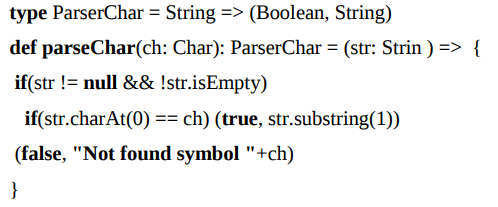
\includegraphics[width=0.7\textwidth]{Smolina/pics/parser1.png}
\end{listing}

Для того чтобы получить синтаксический анализатор подстроки, можно воспользоваться общим подходом и использовать парсер-комбинатор,
который бы составлял в последовательность уже готовые синтаксические анализаторы символов, так называемый парсер-комбинатор последовательности seq. На листинге~\ref{parserSeq} приведен пример реализации.

\begin{listing}
\caption{Парсер-комбинатор последовательности}
\label{parserSeq}
\centering
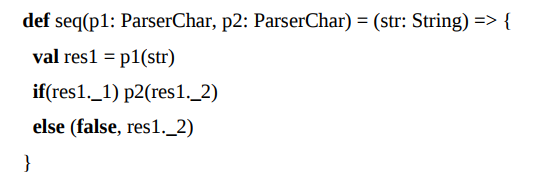
\includegraphics[width=0.7\textwidth]{Smolina/pics/parserSeq.png}
\end{listing}

Теперь, чтобы получить синтаксический анализатор, начинающийся с подстроки “ABC”, мы можем воспользоваться элементарным синтаксическим анализатором символа и парсер-комбинатором последовательности (см. листиниг~\ref{parserABC}).

\begin{listing}
\caption{Парсер-комбинатор строки “ABC”}
\label{parserABC}
\centering
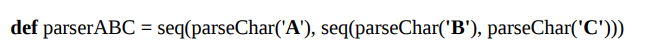
\includegraphics[width=0.9\textwidth]{Smolina/pics/parserABC.png}
\end{listing}

Простые парсер-комбинаторы, основанные на рекурсивном спуске, представляют собой интуитивно ясную модель и поэтому удобны для
отладки. Однако они имеют экспоненциальную сложность по отношению к грамматике~\cite{Popov}. Это связано с тем, что в наивной реализации рекурсивного спуска при откате не сохраняются результаты и таким образом разбор одного и того же символа одним и тем же синтаксическим анализатором может происходить многократно. Решением такой проблемы является мемоизация~\cite{Memoization}. Идея заключается в том, чтобы хранить и переиспользовать результаты примененного синтаксического анализатора для каждого символа входного потока. Таким образом каждое вычисление происходит один раз и в дальнейшем результаты переиспользуются.

 Другой проблемой, ассоциируемой с парсер-комбинаторами, является невозможность обработки леворекурсивных определений анализаторов. Например, грамматика $G_2$ на листиниге~\ref{grmG2}.

 \begin{listing}
\caption{Грамматика $G_2$}
\label{grmG2}
\centering
$\begin{array}{rl}
E \rightarrow E \ + \ a \ | \ a
\end{array}$
 \end{listing}

 В примере синтаксический анализ произвольной строки относительно данной грамматики никогда не завершится, потому что будет происходить бесконечный спуск и ни один символ так и не будет считан из входной строки. 

 Данная проблема имеет несколько решений, одно из которых основано на ограничении числа вызовов нетерминала некоторой константой, например связанной с длиной входной последовательности ~\cite{ParserComb}. Идея решения заключается в том, чтобы для каждого символа последовательности хранить счетчик, который означает сколько раз данный символ был использован распознавателем. Такой счетчик должен быть не больше длины суффикса, который требуется разобрать. Однако, у данного подхода есть недостаток. Во-первых, длина последовательности не всегда известна, например при считывании символов с сетевого сокета. Во-вторых, такой подход обладает сложностью $O(n^4)$, вместо ожидаемой $O(n^3)$, где n – длина последовательности. Подобные проблемы решаются техникой Continuation Parsing Style (CPS) ~\cite{MemoizationInTopDown}. В отличие от первого метода, цепочка леворекурсивных вызовов завершается, когда происходит второй вызов синтаксического анализатора в данной позиции входа. Затем результаты для леворекурсивных синтаксических анализаторов эффективно вычисляются в цикле: пока создается новый результат, завершенные пути синтаксического анализа, записанные как продолжения, перезапускаются в новой входной позиции. Как результат, обработка рекурсивных правил более эффективна и не требует знания длины последовательности. Более подробно об этом речь пойдет в следующей главе.


